%%%%%%%%%%%%%%%%%%%%%%%%%%%%%%%%%%%%%%%%%%%%%%%%%%%%%%%%%%%%%%%%%
% Tese de Doutorado / Dept. Fisica, CFM, UFSC                   %
% Lacerda@CórregoGrande - Jan/2018                              %
%%%%%%%%%%%%%%%%%%%%%%%%%%%%%%%%%%%%%%%%%%%%%%%%%%%%%%%%%%%%%%%%%

%:::::::::::::::::::::::::::::::::::::::::::::::::::::::::::::::%
%                                                               %
%                          Capítulo 4                           %
%                                                               %
%:::::::::::::::::::::::::::::::::::::::::::::::::::::::::::::::%

%***************************************************************%
%                                                               %
%                        DIG discussion                         %
%                                                               %
%***************************************************************%

\chapter{Discussão}
\label{sec:DIGdisc}

Nosso método de classificação é inspirado em argumentos teóricos e empíricos possui diversos propósitos. Neste capítulo vamos aplicar nosso méotodo para nossa amostra do CALIFA cobrindo alguns objetivos específicos:
\begin{enumerate*}[label=(\roman*)]
    \item estimar a relevância do hDIG, mDIG e SFc sobre galáxias cobrindo toda a sequência de Hubble;
    \item estudar a natureza da emissão difusa extraplanar nos sistemas {\em edge-on};
    \item comparar resultados obtidos com o nosso método frente aqueles que separam SF/DIG baseados em um limite fixo em $\Sigma_{\Ha}$;
    \item investigar a possibilidade de discernimento entre regimes DIG e SF baseados em razões de linhas sensíveis à densidade do meio;
    \item testar a consistência de nosso sistema de classificação analisando através de um diagrama clássico de linhas de emissão;
    \item examinar a mistura presente no mDIG;
    \item fechamos a discussão com uma discussão sobre os possíveis {\em caveats} em nosso estudo.
\end{enumerate*}

\section{A relevância das componentes hDIG, mDIG e SFc}
\label{sec:DIGdisc:relstrenghts}

%---------------------------- Figure ----------------------------
\begin{figure}
 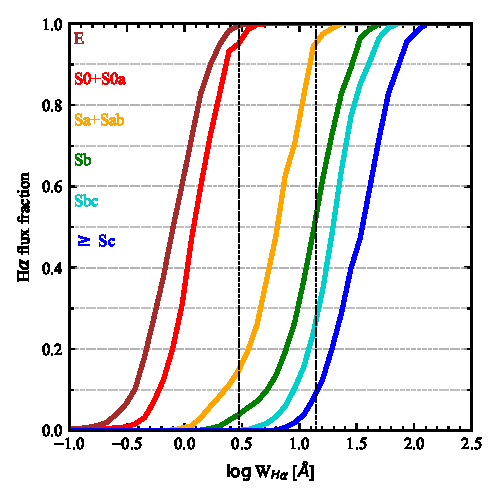
\includegraphics{figuras/fig_cumul_fHaWHa_per_morftype.pdf}
 \caption[Fração cumulativa do fluxo de ${\rm H}\alpha$ com o crescimento de $W_{{\rm H}\alpha}$ para diferentes classes morfológicas]
 {Fração cumulativa do fluxo total de \Ha provenientes de regiões com $W_{\Ha}$ menor que determinado valor. O gráfico mostra as curvas medianas obtidas para galáxias presentes em cada uma de nossas seis classes morfológicas.}
 \label{fig:CurveOfGrowth}
\end{figure}
%---------------------------- Figure ----------------------------

Dentre as questões que podemos perscrutar neste estudo, a importância relativa das componentes de nossa classificação talvez seja a mais importante. A dominância e a evolução da influência que cada um dessas componentes tem sobre galáxias através de diferentes tipos morfológicos é importante na interpretação de propriedades derivadas de dados espectrais não resolvidos espacialmentes. Nesses estudos as assinaturas de regimes distintos vêm todas misturadas sob o mesmo espectro.

Uma maneira simples e relevante observacionalmente de quantificar isso é calculando a contribuição relativa de cada componente para o fluxo total de \Ha. Por exemplo, nas galáxias na Figura \ref{fig:ExampleMaps} essas frações vão de $(f_{\rm hDIG} , f_{\rm mDIG} , f_{\rm SFc}) = (87,13,0)$ para a galáxia S0 CALIFA 0072, até $(5.5,47,47.5)$ para a galáxias Sb CALIFA 0010, e $(0.3,46.1,53.6)$ para a CALIFA 0813, uma Sbc. Essa progressão ao longo da sequência de Hubble reflete as tendências que podem ser vistas na Figure \ref{fig:WHaDistrib_ALLgals}. No canto superior direito de cada painel temos os valores de $(f_{\rm hDIG} , f_{\rm mDIG} , f_{\rm SFc})$ para diferentes distâncias radiais e diferentes tipos morfológicos.

De maneira mais elaborada, a Figura \ref{fig:CurveOfGrowth} mostra essas frações para toda a amostra através dos valores medianos de cada classe morfológica. Nós calculamos a fração cumulativa do fluxo de \Ha, $f$, proveniente de regiões que possuem $W_{\Ha}$ menor que determinado valor. As curvas de $f(<W_{\Ha})$ representam como a fração cumulativa cresce com relação a $W_{\Ha}$. Na figura mostramos as curvas medianas para as nossas seis classes morfológicas. As linhas tracejadas verticais representam nossas fronteiras hDIG/mDIG e mDIG/SFc, em 3 e 14 \AA\ respectivamente.

A progressão constante de {\em early-} para {\em late-type} nessas curvas confirmam nossas expectativas provenientes das distribuições de $W_{\Ha}$ (Figura \ref{fig:WHaDistrib_ALLgals}) além de também nos permitir quantificar a importância relativa entre as componentes e o fluxo total de \Ha. Em galáxias elípticas ou S0 temos praticamente toda a emissão de \Ha na fase hDIG ($W_{\Ha} \le 3$). Entre os sistemas Sa-Sab, essa componente se encarrega por 14\% do fluxo de \Ha, com o mDIG sendo o responsável por praticamente todo o fluxo restante. De Sb para frente, o regime SFc domina, sendo responsável por 50\% ou mais. Natualmente existe um espalhamento natural nos dados, mesmo quando divididos em classes morfológicas.

A contribuição relativa do DIG para a emissão em \Ha foi estimada em diversos estudos anteriores, geralmente baseados em dados obtidos com filtros estreitos (\Ha + \nii) \citep{Ferguson.etal.1996, Zurita.etal.2000, Thilker.etal.2002, Oey.etal.2007}, com resultados variando substancialmente principalmente devido a diferenças na metodologia de separação da emissão difusa. O maior estudo até hoje foi feito por \citet{Oey.etal.2007}, que estimaram a fração de emissão difusa em \Ha de $59\pm19 \%$ sobre uma amostra de 109 galáxias do {\em survey} SINGG \citep{Meurer.etal.2006}. Para nossa amostra (e nossas definições) nós encontramos um valor bem próximo, 56\% (hDIG + mDIG), mas com um espalhamento muito maior, $\pm38 \%$. Diferentemente de nosso estudo (Figura \ref{fig:CurveOfGrowth}), eles não encontraram nenhuma evidencia de correlação com o tipo morfológico. Talvez o motivo seja devido a diferença de critério e metodologia de classificação DIG/SF.


\section{Emissão extraplanar em sistemas {\em edge-on}}
\label{sec:DIGdisc:edgeon}

%---------------------------- Figure ----------------------------
\begin{figure}
 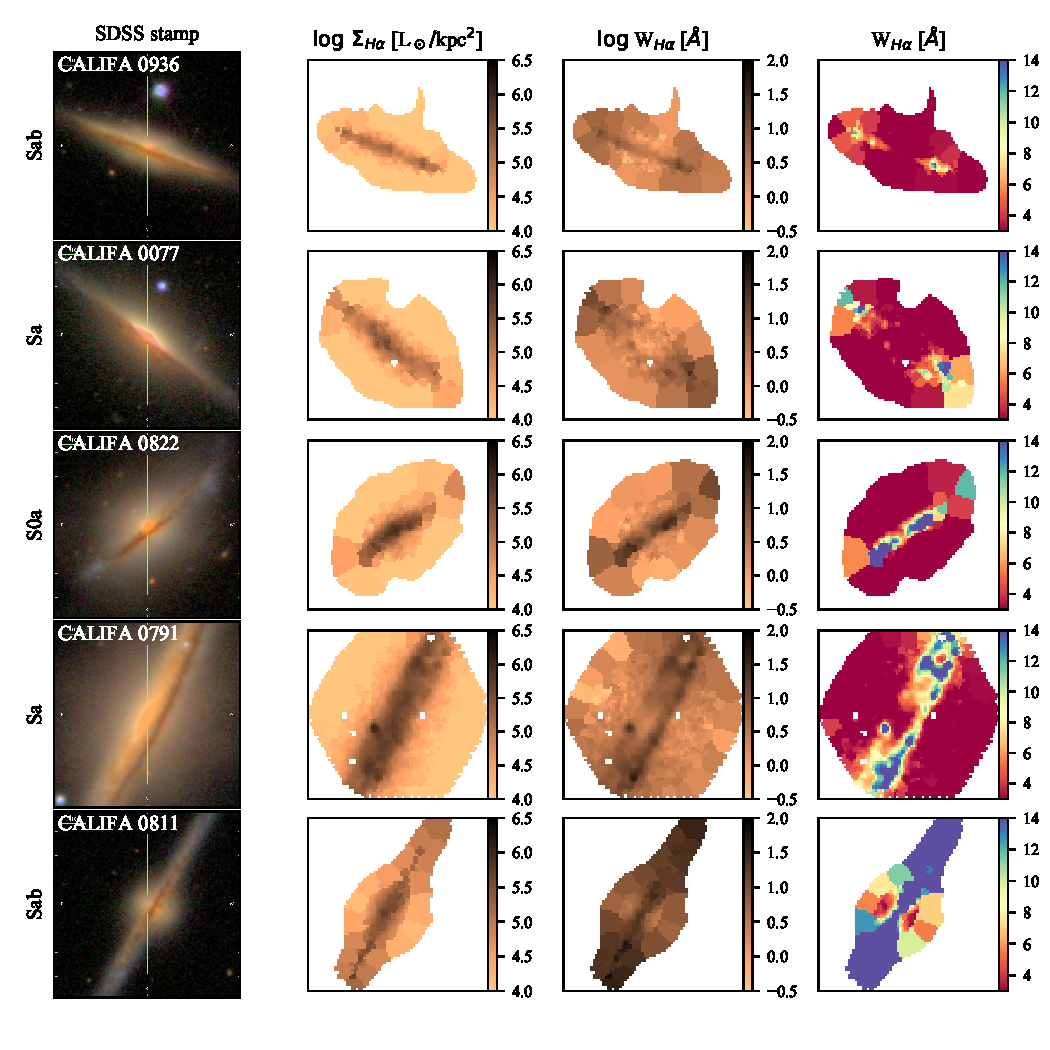
\includegraphics{figuras/fig_maps_class_edgeon_paper.pdf}
 \caption[Imagem \SDSS e mapas de $\Sigma_{{\rm H}\alpha}$ e $W_{{\rm H}\alpha}$: sistemas {\em edge-on}]
 {Como a Figura.\ \ref{fig:ExampleMaps}, mas para galáxias {\em edge-on}.}
 \label{fig:ExampleMapsEdgeOn}
\end{figure}
%---------------------------- Figure ----------------------------

Devido ao comportamento sistemático das propriedades de linhas de emissão, esses sistemas altamente inclinados são importantes para o estudo da emissão DIG nas regiões acima (e abaixo) do disco galáctico \citep{Tullmann.and.Dettmar.2000, Otte.etal.2002, Jones.etal.2017}. A galáxia protótipo utilizada nesses estudos é a NGC 891, extensivamente observada em diversos comprimentos de onda \citep{Rand.1998, Hodges.and.Bregman.2013, Seon.etal.2014, Hughes.etal.2015}. Esses estudos enfatizaram que as propriedades de linhas de emissão observadas no DIG extraplanar não podem ser explicadas puramente por fótons Lyman que escapam de regiões \hii presentes no disco. Uma variedade de fenômenos que pudessem gerar tal emissão foram sugeridos, como: dissipação de turbulência \citep{Minter.and.Spangler.1997}, reconexão magnética \citep{Raymond.1992}, choques \citep{Collins.and.Rand.2001}, raios cósmicos, aquecimento fotoelétrico proveniente de grãos de poeira do meio interestelar  \citep{Weingartner.and.Draine.2001}, e fótons Lyman vindos de estrelas velhas e quentes \citep{FloresFajardo.etal.2011a}.

A Figura \ref{fig:ExampleMapsEdgeOn} nos mostra como os dados do CALIFA podem nos trazer um novo {\em insight} ao problema. Nela vemos cinco exemplos de galáxias {\em edge-on} dispostas da mesma forma que na Figura \ref{fig:ExampleMaps}. As quatro primeira possuem configuração muito parecida, onde temos o disco e arredores dominados por mDIG e SFc, enquanto a grandes distâncias do disco galácticos vemos uma completo predomínio de hDIG. Isso favorece o cenário proposto por \citet{FloresFajardo.eteal.2011a}, onde a ionização se torna dominada por HOLMES à medida que nos afastamos do plano galáctico. Essa conclusão é reforçada pelos mapas de diagnóstico de razões de linhas baseados em dados do MaNGA em \citet{Belfiore.etal.2016} e \citet{Zhang.etal.2017a}.

Através de nossa experiência calculando $\xi$ (veja a Seção \ref{sec:DIGclass:WHaDistrib_hDIG}) podemos, pela primeira vez, relacionar a emissão DIG extraplanar com as populações estelares subjacentes. A mediana de $\xi$ nas regiões extraplanares das quatro primeiras galáxias na Figura \ref{fig:ExampleMapsEdgeOn} é 1.5 com interquartis 1.1--1.9. Dado um fator de $2 \sim 3$ nessa estimativa \citep{CidFernandes.etal.2011a} a conclusão principal aqui é que $\xi$ é da ordem de 1 e por isso consegue produzir fótons com $h\nu > 13.6$ suficientes para explicar a emissão extraplanar de \Ha.

Se essas galáxias fossem vistas {\em face-on}, o DIG extraplanar estaria projetado por cima do disco, que é dominado por mDIG + SFC. Para uma emissividade constante de \Ha, a razão entre $\Sigma_{\Ha}$ {\em face-on} e {\em edge-on} é igual a razão entre $h/r$ (altura e raio) da camada hDIG extraplanar. Nas galáxias da Figura \ref{fig:ExampleMapsEdgeOn} o valor de $\Sigma_{\Ha}$ é de aproximadamente algumas vezes $10^4 L_\odot\,$kpc$^{-2}$. Para $h \sim r$, este também deve ser o brilho superficial dessa componente. Esse valor é muito menor que os que estão presentes nas regiões SFc das galáxias {\em face-on} da Figura \ref{fig:ExampleMaps}, nesse caso, portanto, o efeito do hDIG extraplanar projetado pode ser negligenciado. Porém, algumas regiões mDIG apresentam valores não muito maiores que $10^4 L_\odot\,$kpc$^{-2}$ podendo assim carregar alguma contribuição não-negligenciável do hDIG extraplanar.

A galáxia na última linha da Figura \ref{fig:ExampleMapsEdgeOn} (CALIFA 0811, UGC 10043) é diferente das demais, como podemos ver pelo seu mapa de classificação. Ela possui muito mais SFc no seu disco e em regiões extraplanares, além de um cone bipolar com valores intermediários de $W_{\Ha}$ centrado no núcleo. Essa galáxia foi recentemente estudada por \citet{LopezCoba.etal.2017}, no qual encontraram razões entre linhas de emissão e cinemática consistentes com vento galáctico alimentado por um evento SF central. Essa combinação de ionização por choque e formação estelar espalhada pelo disco explica porque não há emissão hDIG extraplanar nessa galáxia, embora seja curioso que os valores de $W_{\Ha}$ caiam para valores hDIG nas partes internas do bicone.


\section{Comparações com esquemas de separação SF/DIG baseados em $\Sigma_{{\rm H}\alpha}$}
\label{sec:DIGdisc:compSBHa}

%---------------------------- Figure ----------------------------
\begin{figure}
 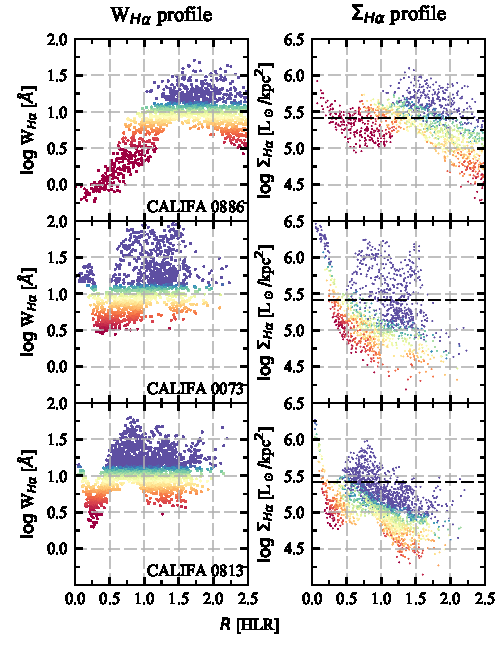
\includegraphics[scale=1.7]{figuras/fig_WHaSBHa_profile_faceon_paper.pdf}
 \caption[Perfis radiais de $W_{{\rm H}\alpha}$ e $\Sigma_{{\rm H}\alpha}$]
 {Perfis radiais de $W_{{\rm H}\alpha}$ e $\Sigma_{{\rm H}\alpha}$ para três galáxias presentes na Figura \ref{fig:ExampleMaps}. Os pontos são coloridos segundo $W_{\Ha}$. As linhas pontilhadas nos painéis da direita marcam $\Sigma_{\Ha} = 10^{39}$ erg$\,$s$^{-1}\,$kpc$^{-2}$.}
 \label{fig:WHa_and_SHa_profiles}
\end{figure}
%---------------------------- Figure ----------------------------

Apesar das vantagens conceituais desse modo de classificação apresentado até agora, $W_{\Ha}$ possui $\Sigma_{\Ha}$ no seu numerador, por isso pode-se imaginar que um modelo de classificação baseado nessas duas variáveis deveriam ter resultados semelhantes. Através dos mapas da Figura \ref{fig:ExampleMaps} podemos perceber que algumas estruturas, como os braços de formação estelar, são concomitantemente identificados por $W_{\Ha}$ e $\Sigma_{\Ha}$, porém outras não são. Mais precisamente, $\Sigma_{\Ha}$ sempre tem um máximo no centro da galáxia, porém, para galáxias {\em early-type}, $W_{\Ha}$ mostra evidentes declives.

Três exemplos de galáxias presentes na Figura \ref{fig:ExampleMaps}, CALIFA 0886, 0073 e 0813, com seus respectivos perfis radiais de $W_{\Ha}$ e $\Sigma_{\Ha}$ aparecem na Figura \ref{fig:WHa_and_SHa_profiles}. (Exemplos de perfis radiais como esses podem ser encontrados em \citealt{Papaderos.etal.2013, Belfiore.etal.2016, Belfiore.etal.2017, Gomes.etal.2016b, GonzalezDelgado.etal.2016a}.) Na coluna da esquerda (direita) temos os valores de $W_{\Ha}$ ($\Sigma_{\Ha}$) contra R. Ambos são coloridos por $W_{\Ha}$ segundo o mesmo esquema de cores utilizado até aqui.

A CALIFA 0886 é um bom exemplo de galáxia que apresenta valores baixos de $W_{\Ha}$ em seu centro dominado por emissão hDIG, porém com um pico em $\Sigma_{\Ha}$ nessa mesma região. A alta concentração de HOLMES no bojo da galáxia faz com que o mesmo seja muito mais brilhante que o disco que o cinge. O aumento do brilho superficial de \Ha devido a geometria do bojo pode fazer com que essa emissão seja incorretamente classificada como SF quando utilizamos um esquema de classificação SF/DIG baseados em $\Sigma_{\Ha}$. Como vemos no painel do topo à direita, os valores de $\Sigma_{\Ha}$ estão acima da linha pontilhada, que marca o limite que seleciona confiávelmente spaxels dominados por regiões \hii segundo \citet{Zhang.etal.2017a}, $\Sigma^{\rm SF,min}_{\Ha} = 10^{39}$ erg$\,$s$^{-1}\,$kpc$^{-2} =  2.6 \times 10^{5} L_\odot\,$kpc$^{-2}$. No entanto, vemos que as mesmas regiões possuem $W_{\Ha} \sim 1$ \AA, sem dúvidas operando sob regime hDIG. O critério utilizando $W_{\Ha}$ corretamente classifica o bojo dessa e de outras galáxias como aposentado, enquato um critério baseado em $\Sigma_{\Ha}$ os interpretaria como dominados por regiões SF.

%---------------------------- Figure ----------------------------
\begin{figure}
 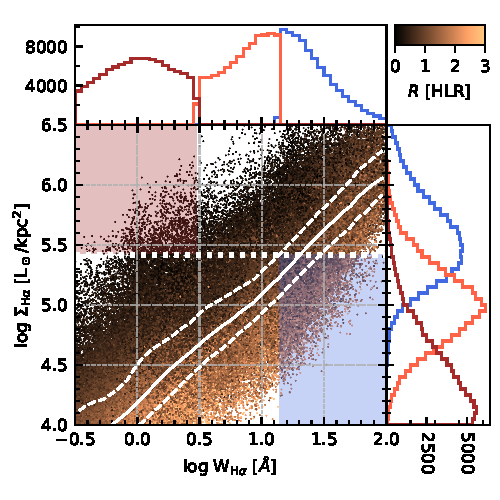
\includegraphics[scale=1.5]{figuras/fig_logSBHa_logWHa_histograms.pdf}
 \caption[$\log \Sigma_{{\rm H}\alpha} \times \log W_{{\rm H}\alpha}$]
 {$\log \Sigma_{\Ha}$ em função de $W_{\Ha}$ para as zonas de nossa amostra. Os intervalos em ambos eixos estão limitados àqueles valores que utilizamos para saturar os mapas na Figura \ref{fig:ExampleMaps}. Os pontos estão coloridos conforme a distânciada até o núcleo (em unidades de HLR). Os histogramas de $\Sigma_{\Ha}$ e de $W_{\Ha}$ estão coloridos com as mesmas cores utilizadas naqueles na Figura \ref{fig:WHa-Xi}. A linha contínua e as linhas tracejadas em branco marcam a mediana e o intervalo interquartil respectivamente. O limite $\Sigma^{\rm SF,min}_{\Ha} = 10^{39}$ erg$\,$s$^{-1}\,$kpc$^{-2}$ proposto por \citet{Zhang.etal.2017a} é sinalizando utilizando uma linha horizontal pontilhada branca. Um retângulo vermelho com bolas representa regiões classificadas como hDIG que possuem brilho superficial acima desse limite. Já aquelas regiões classificadas como SFc abaixo desse limite estão sobre um retângulo azul com estrelas.}
 \label{fig:logWHa_logSBHa_histo}
\end{figure}
%---------------------------- Figure ----------------------------

Ao longo do disco da CALIFA 0886 a classificação utilizando o limite proposto por \citet{Zhang.etal.2017a} em $\Sigma_{\Ha}$ concorda com o regime nebular identificado por $W_{\Ha}$. Essa concordância ocorre apenas de forma parcial na CALIFA 0073 (painéis centrais na Figura \ref{fig:WHa_and_SHa_profiles}), onde encontramos mais regiões SF no disco utilizando o critério baseado em $W_{\Ha}$ do que aquele em $\Sigma_{\Ha}$. Esse fato é ainda mais acentuado na CALIFA 0813 (painéis inferiores), onde a maioria das regiões com $W_{\Ha} > 14$ \AA\ possuem $\Sigma_{\Ha}$ abaixo do limite $\Sigma^{\rm SF,min}_{\Ha}$. Essas diferenças se originam nos comportamentos radiais distindos entre $\Sigma_{\Ha}$ e $W_{\Ha}$.

Na Figura \ref{fig:logWHa_logSBHa_histo} podemos ver tudo isso de forma estatística. Os pontos representam as zonas em nossa amostra, coloridos por $R$. Vemos que para um valor de $W_{\Ha}$, as regiões mais brilhantes (maior $\Sigma_{\Ha}$) estão localizadas nas regiões centrais. Já para um valor fixo de $\Sigma_{\Ha}$, os maiores valores de $W_{\Ha}$ tendem a estar nos arredores. De fato, como vimos nos exemplos da Figura \ref{fig:WHa_and_SHa_profiles}, $\Sigma_{\Ha}$ tende a diminuir enquanto $W_{\Ha}$ se mantém mais ou menos constante, ambos com grandes dispersões em qualquer $R$ no disco. Cerca de 37\% das nossas regiões SFcc possuem $\Sigma_{\Ha} < 10^{39}$ erg$\,$s$^{-1}\,$kpc$^{-2}$. Na média, essas regiões SFc pouco brilhantes estão localizadas em $R = 1.3$ HLR.

A área pintada em azul com estrelas na Figura \ref{fig:logWHa_logSBHa_histo} marca regiões em que $\Sigma_{\Ha} < \Sigma^{\rm SF,min}_{\Ha}$, porém com $W_{\Ha} > 14$ \AA, como vemos nos discos da CALIFA 0073 e na 0813. Se apoiando no exemplo da CALIFA 0886, vemos na área vermelha com bolas, regiões que seriam classificadas erroneamente utilizando o limite baseado em $\Sigma_{\Ha}$ proposto por \citet{Zhang.etal.2017a}. Também podemos ver nessas áreas pintadas, agora com relevância estatística, esses casos onde regiões SFc com baixo brilho nas estão geralmente situadas nas regiões exteriores e regiões dominadas pelo regime hDIG, porém muito brilhantes, situadas em $R < 1$.

Em resumo, comparado com o método de classificação em hDIG/mDIG/SFc baseado em $W_{\Ha}$ proposto neste trabalho, um critério baseado em $\Sigma_{\Ha}$ tente a sobrestimar a população de regiões SF situadas nas regiões mais internas das galáxias. De maneira mais critica, como já foi mencionado, $\Sigma_{\Ha}$ não pode, por si, identificar a componente hDIG, maior fonte de emissão em \Ha em velhos esferóides. Realmente temos visto que bojos aposentados ({\em retired bulges}) muitas vezes são classificados como SFc quando o brilho excede $\Sigma^{\rm SF,min}_{\Ha}$.

Trabalhos anteriores de utilizando dados do CALIFA por \citet{Kehrig.etal.2012}, \citet{Singh.etal.2013}, e \citet{Gomes.etal.2016b} também encontram valores $\Sigma_{\Ha}$, acima do limite $\Sigma^{\rm SF,min}_{\Ha}$ proposto por \citet{Zhang.etal.2017a}, nas regiões internas de galáxias {\em early-type}, onde incontestavelmente existe a ausência de estrelas jovens. (Veja também \citealt{Sarzi.etal.2010} para resultados baseados nos dados do SAURON\footnote{\em Spectrographic Area Unit for Research on Optical Nebulae survey}). Esses exemplos são realizações observacionais da inconsistência conceitual da soma de regiões DIG resultar em uma errônea classificação SF, apontada na Seção \ref{sec:DIGclass:WHaDistrib_hDIG}. O esquema apresentado nesta tese resolve esse problema extendendo para uma análise espacialmente resolvida, o conceito de galáxias aposentadas proposta por \citet{Stasinska.etal.2008a} e \citet{CidFernandes.etal.2011a} no contexto de espectros integrados.


\section{O DIG pode ser identificado por razões de linha sensíveis à densidade do meio?}
\label{sec:DIGdisc:nSii}

%---------------------------- Figure ----------------------------
\begin{figure}
 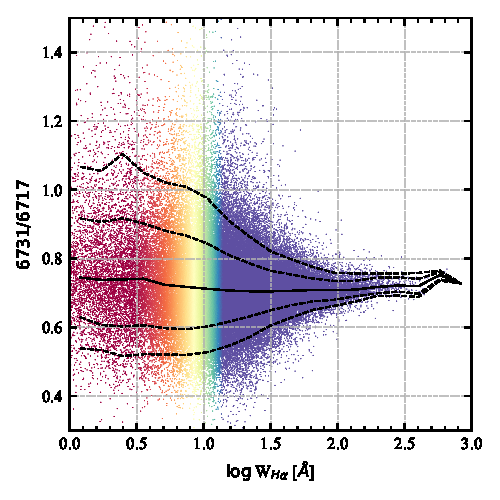
\includegraphics{figuras/fig_SII_logWHa_SNR3.pdf}
 \caption[$\log$ \sii$\times \log W_{{\rm H}\alpha}$]
 {Razão do fluxo de [S\,{\sc ii}]$\lambda\lambda$6731/6716 para $111\,760$ zonas em nossa amostra nas quais essa razão tem relação SN $\ge 3$. Pontos estão coloridos por $W_{\Ha}$ como nas figuras anteriores. A linha sólida representa a curva mediana, enquanto linhas tracejadas mostram os intervalos equivalentes a 1 e $2\sigma$ respectivamente.}
 \label{fig:S2_WHa}
\end{figure}
%---------------------------- Figure ----------------------------

As densidades eletrônicas do DIG na Via Láctea, obtidas através da combinação de medidas de dispersão e emissão e das colunas de densidade de \hi na direção de pulsares com distâncias conhecidas, são tipicamente abaixo de $10^{-1}$ cm$^{-3}$ \citep{Berk.and.Fletcher.2008}, ordens de magnitude menores que aqueles para regiões \hii. Poderíamos então pensar que uma estudo espacialmente resolvido da razão de linhas \Sii\ indicaria uma menor densidade nas regiões de DIG do que nos SFc. Nesse caso, tal razão mostraria uma tendência com $W_{\Ha}$. As linhas do \sii resultam da população através de excitação colisional de níveis muito próximos energeticamente e a razão da população dos níveis energéticos é proporcional à densidade do meio. Restringimos nossa amostra àquelas zonas onde SN $\ge 3$ na razão de linha \sii e mostramos na Figura \ref{fig:S2_WHa} a razão \sii 6731/6716 em função de $W_{\Ha}$. Nela vemos a curva mediana e os intervalos de 1 e 2$\sigma$ plotados. Não pudemos encontrar nenhuma relação entre a razão \sii 6731/6716 e $W_{\Ha}$. O aumento no espalhamento de pontos na direção de baixos $W_{\Ha}$ é consistente com a queda na relação SN das linhas. Mesmo nas regiões onde essa razão pode ser medida com segurança seu valor é $\sim 0.7$, limite inferior (baixa densidade) do intervalo sensível à densidade eletrônica através da razão \sii. Claro que essa figura não pode falar nada para as regiões onde SN < 3.

Nossa interpretação é que a razão de linhas \sii não nos mostra uma diferença quantitativa entre regiões DIG que puderam ter \sii medido e aquelas sob regime SFc por duas razões:
\begin{enumerate*}[label=(\roman*)]
    \item na resolução de nossos dados, as regiões SFc contém uma quantidade significativa de gás difuso;
    \item a razão de linhas \sii não é sensitiva à densidades menores de $\sim 50$\,cm$^{-3}$.
\end{enumerate*}

Poderíamos imaginar que um cenário diferente se formaria com estudos utilizando um dubleto sensitivo a baixas densidades, como o \Nii presente no infravermelho distante. Observações recentes mapearam essa razão na Via Láctea e outras galáxias \citep{Goldsmith.etal.2015, HerreraCamus.etal.2016}. As densidades derivadas estão no intervalo de 1 a 300 cm$^{-3}$ com um valor mediano de 30 cm$^{-3}$. Esses valores não chegam perto das densidades do DIG obtidas por medidas através de pulsares.

Portanto concluímos que estimadores clássicos de densidade não são hábeis para detectar o DIG, pelo menos não na resolução do CALIFA ou {\em surveys} simliares. Entretanto, não é bem certo se eles farão um melhor trabalho sob resolução espacial melhor pois, como percebido por \citet{Rubin.1989} sob outro contexto, inomogeneidades na densidade dificultam profundamente qualquer interpretação qualitativa de tais razões de linhas sensitivas à densidade do meio.


\section{$W_{{\rm H}\alpha}$ e o diagrama BPT}
\label{sec:DIGdisc:BPT}

%---------------------------- Figure ----------------------------
\begin{figure}
 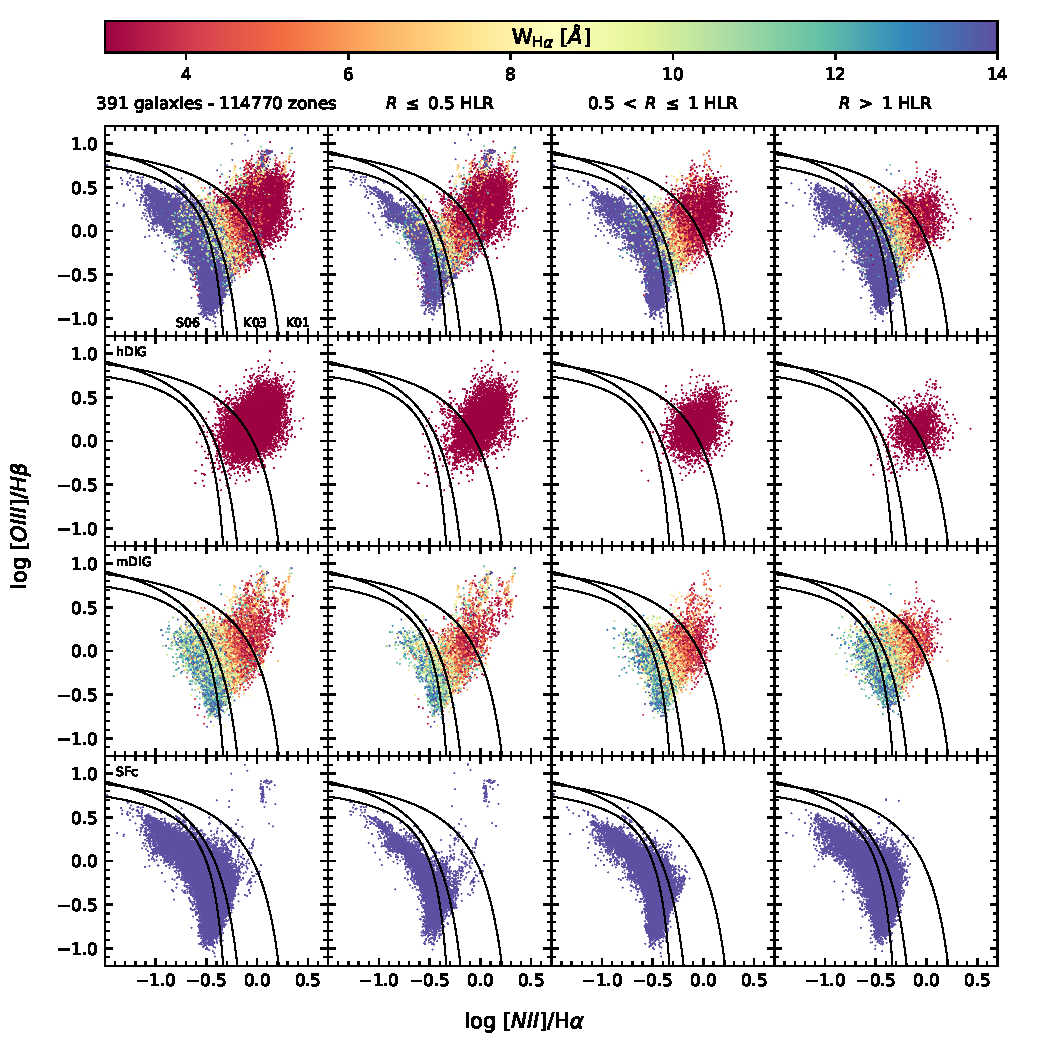
\includegraphics[scale=0.85]{figuras/fig_BPT_per_R.pdf}
 \caption[Diagramas BPT]
 {Diagrama BPT para nossa amostra. A primeira linha mostra todas as regiões em nossa amostra. Demais linhas dividem a amostra entre regiões SFc ($W_{\Ha} > 14$ \AA), mDIG ($W_{\Ha} = 3$--14 \AA), e hDIG ($W_{\Ha} < 3$ \AA). Em todos os painéis os pontos coloridos por $W_{\Ha}$ como indicado. Enquanto na primeira coluna temos os pontos para todas as posições das galáxias, nas seguintes os pontos são classificados de acordo com suas distâncias radiais, $R$, como na Figura \ref{fig:WHaDistrib_ALLgals}. Em todos os casos, plotamos apenas zonas com $SN \ge 3$ nas quatro linhas envolvidas. As curvas divisoras vêm de \citet[S06]{Stasinska.etal.2006a}, \citet[K03]{Kauffmann.etal.2003a}, e \citet[K01]{Kewley.etal.2001a} respectivamente.}
 \label{fig:BPT}
\end{figure}
%---------------------------- Figure ----------------------------

Diferentes processos de aquecimento e regimes de ionização no hDIG, mDIG e SFc devem resultar em diferentes razões entre fluxos de linhas colisionais e de recombinação, portanto distintas posições em diagramas de excitação como o  \Oiii/\Hb versus\ \Nii/\Ha. Esse famoso diagrama BPT \citep*[após][]{Baldwin.Phillips.Terlevich.1981a} é amplamente utilizado para separar galáxias SF daquelas onde uma fonte de ionização mais dura contribui de forma significante para a ionização do gás. Uma maneira de caracterizar regimes nebulares de forma independente serve de palco ideal para um teste de consistência da nossa classificação baseada em $W_{\Ha}$.

A Figura \ref{fig:BPT} mostra o diagrama BPT obtido para todas as zonas onde SN $\ge 3$ nas quatro linhas envolvidas. Os dados estão distribuídos de forma em que na coluna mais à esquerda estejam presentes regiões espalhadas em todas as partes das galáxias. Demais colunas separam regiões em três intervalos de distância radial como na Figura \ref{fig:WHaDistrib_ALLgals}. Na primeira linha vemos toda a amostra e, nas seguintes, os dados divididos entre hDIG/mDIG/SFc. Em todos os painéis os pontos são coloridos por $W_{\Ha}$ seguindo o mesmo esquema utilizado nos painéis da coluna da direita na Figura \ref{fig:ExampleMaps}. As curvas plotadas são aquelas propostas por \citet[S06]{Stasinska.etal.2006a}, \citet[K03]{Kauffmann.etal.2003a}, e \citet[K01]{Kewley.etal.2001a}. Essas curvas, teóricas ou empíricas, servem como divisórias demarcando distintos regimes de ionização no plano BPT -- veja \citet{CidFernandes.etal.2011a} para uma discussão sobre o significado dessas curvas.

A forte correspondência entre $W_{\Ha}$ e as coordenadas no BPT é evidente, como foi previamente percebida por \citet{Morisset.etal.2016} com dados do CALIFA e \citet{Belfiore.etal.2016} com o MaNGA. A asa esquerda é predominantemente populada por regiões SFc, enquanto o hDIG se distribui pela a asa direita, principalmente na ponta. Podemos notar que cada uma de nossas classes de regime de ionização preserva a área no plano BPT onde exerce uma predominância relativa, mesmo para diferentes intervalos de distância radial. Os pontos atípicos que aparecem nos dois painéis mais à esquerda na última linha, situados na região do plano BPT que é ocupado particularmente por regiões hDIG, se concentram nas regiões mais internas das galáxias. São regiões de nossa amostra onde $W_{\Ha}$ é alto mas são dominadas por ionização proveniente de um AGN, como será discutido na Seção \ref{sec:DIGdisc:caveats}.

Restringindo nossa análise para pontos onde $R > 1$ HLR (coluna mais à direita) para mitigar contaminação por regiões ionizadas por núcleos ativos, verificamos que 58\% (92\%) de nossas zonas com $W_{\Ha}$ > 14 \AA\ são classificadas como SF de acordo com o critério proposto por S06 (K03). O número relativamente grande de regiões SF que ultrapassam a linha de S06 não é surpreendente, já que a mesma foi traçada utilizando modelos de fotoionização desenvolvidos para estabelecer um limite para regiões puramente ionizadas por formação estelar. Como já argumentamos diversas vezes nesta tese, na resolução do CALIFA nossas regiões SFc não chegam nem perto de serem regiões \hii puras, por isso possuem bastante emissão difusa, o que acaba inflando ambas razões de linhas no diagrama BPT.

Concluímos portanto que nosso esquema de separação hDIG/mDIG/SFc leva a razões de linhas qualitativamente compatíveis com as quais deveríamos esperar em regiões sob tais regimes nebulares. Juntamente com os argumentos conceituais e empíricos apresentados na Seção \ref{sec:DIGclass:WHa}, essa análise utilizando o diagrama BPT adiciona força à nossa metodologia.


\section{O mDIG como uma mistura de SF+hDIG}
\label{sec:DIGdisc:mDIG}

%---------------------------- Figure ----------------------------
\begin{figure}
 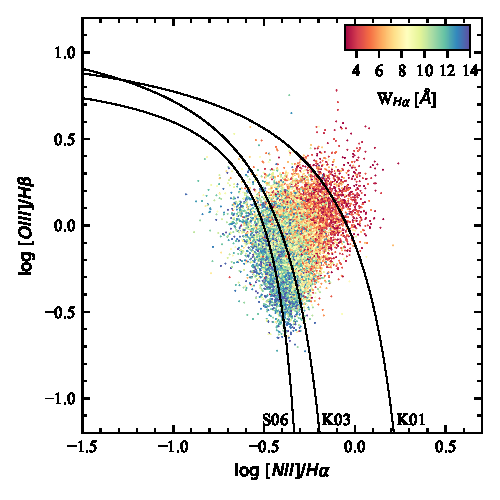
\includegraphics{figuras/fig_BPT_mixed.pdf}
 \caption[Diagrama BPT -- mDIG]
 {Diagrama BPT filtrando apenas regiões mDIG (i.e., aquelas onde $W_{\Ha}$ está no intervalo 3--14 \AA), com pontos coloridos de acordo com $W_{\Ha}$, e excluindo zonas até $R = 1$ HLR.}
 \label{fig:BPT_mDIG}
\end{figure}
%---------------------------- Figure ----------------------------

Esta seção surge como um {\em addendum} à anterior, com a finalidade de explorar a natureza de emissão das regiões mDIG. A forma com que as regiões mDIG (penúltima linha da Figura \ref{fig:BPT}) se distribuem no diagrama BPT, entre a asa clássica das regiões SF e o local predominantemente populado por regiões hDIG, leva a uma interpretação em termos de uma mistura de fenômenos.
%Esse comportamento, por si só, já nos estimula a evocar tal cenário, porém podemos dizer mais utilizando o diagrama BPT.
A Figura \ref{fig:BPT_mDIG} trás em destaque o painel mais à direita da penúltima linha da Figura \ref{fig:BPT}. Nela vemos os pontos associados às regiões mDIG situadas em $R\ > 1$ HLR (= 5.3 kpc na média), coloridos por $W_{\Ha}$ como indicado.

A mesma progressão regular de $W_{\Ha}$ observada no painel do topo à esquerda na Figura \ref{fig:BPT} é observada na Figura \ref{fig:BPT_mDIG}, sugerindo fortemente um cenário composto pela mistura de emissão SFc e hDIG. A população de regiões mDIG com $W_{\Ha}$ perto do limite de 14 \AA\ provavelmente corresponde a um cenário ionização devido ao escape de fótons de regiões SFc. De fato esses pontos se sobrepõem às coordenadas do BPT dominada por SFc. Acima da asa SF do BPT, o processo de ionização continua sendo principalmente governado por estrelas jovens e massivas, porém a influência do aquecimento por HOLMES aumenta gradativamente enquando $W_{\Ha}$ diminui. Quando $W_{\Ha}$ chega próximo ao limite de 3 \AA, o campo de radiação ionizante gerado por HOLMES começa a dominar o processo de fotoionização.


%\section{AGN e outros {\em caveats}}
\section{AGN e outras fontes de linhas de emissão}
\label{sec:DIGdisc:caveats}

Nosso método de classificação hDIG/mDIG/SFc ignora outros mecanismos de produção de linhas. Dentre eles, o AGN é o mais notável. AGNs são encontrados nas partes centrais de galáxias e reconhecíveis através do diagrama BPT. Por exemplo, os pontos na ponta da asa direita com $W_{\Ha} > 14$ \AA\ na Figura \ref{fig:BPT} são provenientes das regiões internas da galáxias CALIFA 0897 (UGC 12348), um tipo conhecido de Seyfert tipo 2 \citep{Cusumano.etal.2010, Asmus.etal.2014}. Notamos que outros pontos erráticos que possuem $W_{\Ha} > 3$ e situados em regiões internas ($R$ pequeno) tendem a ocupar a área do BPT geralmente ocupado por regiões hDIG.

AGNs podem prover energia para emissão de linhas em regiões muito distantes do núcleo (até distâncias de 20kpc; \citealt{Veilleux.etal.2003}). Essas são conhecidas como EELRs ({\em extended emission-line regions}) ou cones de ionização. Esses cones podem ser originadas por fotoionização de fótons de raio-X que deixam o núcleo com um pequeno ângulo de abertura ou por interação entre {\em radio jets} e o meio interestelar da galáxias produzindo fortes choques \citep{Wilson.1996}. Entretanto, na linha do presente estudo, o qual é avaliar a importância do DIG em galáxias em pontuar seus diferentes regimes, EELRs em galáxias Seyfert são um problema secundário, pois afetam apenas regiões específicas de galáxias com um AGN bem definido -- e talvez nem todas elas. Entender as EELRs é um tópico de estudo {\em per se} para ser investigado com espectroscopia 3D, e alguns estudos já começaram a fazê-lo \citep[e.g.,][]{Dopita.etal.2014}, porém está fora do escopo desta tese.

Choques estão também entre outros processos que podem gerar linhas de emissão e são negligenciados neste trabalho. No casso do vento galáctico na CALIFA 0811, presente na Figura \ref{fig:ExampleMapsEdgeOn}, encontramos $W_{\Ha}$ = 3--12 \AA\ na área de choque, i.e., valores presentes nas regiões que classificamos como mDIG. Novamente argumentamos que $W_{\Ha}$ por si não pode identificar a origem dessa emissão nebular, apenas que fotoionização por HOLMES não é uma explicação factível. Apenas um estudo detalhado da geometria, razões de linhas e cinemática objetos poderiam revelar os processos que governam a emissão de linhas nesses objetos \citep{Kreckel.etal.2014, Beirao.etal.2015, LopezCoba.etal.2017}. Devido ao seu número relativamente pequeno e por sua limitação espacial, tais objetos também não influenciam muito na estatística hDIG/mDIG/SFc presente neste estudo, entretanto não devem ser negligenciados em estudos individuais.

Finalmente, uma discussão sobre a tão conhecida região composta no BPT diagrama, comumente definida pela região abaixo da linha K01 e acima da K03 ou S06. Os objetos que ali se situam são interpretados geralmente como uma composição de SF + AGN, porém AGN e hDIG possuem razões de linha indistinguíveis em relação ao BPT. Portanto, a priori, não podemos afirmar realmente de que processos essa região é composta.

A forma de quebrar essa degenerescência é através de $W_{\Ha}$. Sabemos que estrelas velhas e quentes, diferentemente de AGN ou SF, ocupam toda a extensão de galáxias.
Consequentemente, o regime hDIG deve ser considerado
%A radiação proveniente dos HOLMES, que produz $W_{\Ha} \sim 1$ \AA, deve portanto ser considerada
nível fundamental de ionização, ou seja, aquele que é energéticamente relevante quando nenhum outro é. Sempre que o contínuo ao redor de \Ha\ for dominado por estrelas velhas, que é o caso mesmo para regiões SF na resolução na casa de {\em kiloparsec}, a razão entre o fluxo ionizante e aquele proveniente do contínuo estelar deve gerar valores de $W_{\Ha} \sim$ 1--2 \AA\ de acordo com os modelos de população estelar (ver \citealt{CidFernandes.etal.2011a} e referências ali). Logo, espectros que possuam $W_{\Ha}$ próximo desse valor e caiam na região composta do BPT certamente representam uma mistura SFc + hDIG. Entretando, enquanto $W_{\Ha}$ estiver acima do intervalo hDIG, uma mistura formada por SF + AGN é mais plausível.

O estudo de \citet{Davies.etal.2014} ilustra este ponto. Usando cubos de dados do CALIFA de quatro galáxias, duas  Seyfert (NGC 2410 e NGC 6394) e outras duas onde a classificação Seyfert--LINER é incerta (IC 0540 e NGC 6762), eles identificam distribuições praticamente unidimensionais no diagrama BPT e outros diagramas de excitação. Essas distribuições sugerem uma sequência de mistura SF + AGN. No entanto eles verificaram que na NGC 6762 a maioria (> 90\%) dos {\em spaxels} possuem $W_{\Ha} < 3$ \AA\ e, por essa razão, a contribuição de HOLMES não pode ser ignorada. Por outro lado, as galáxias NGC 2410 e NGC 6394 possuem regiões centrais com $W_{\Ha}$ bem acima do limite de hDIG, portanto uma mistura SF + AGN é mais provavel. Na IC 0540 os valores de $W_{\Ha}$ estão no intervalo hDIG--mDIG, o qual torna qualquer interpretação sob estes argumentos menos exata, embora eles pendem para uma mais favorável à mistura SF + AGN. Cremos que o ponto principal aqui é que $W_{\Ha}$ deve ser levado sempre em conta em estudos de sistemas compostos a fim de evitarmos confusão entre os efeitos do hDIG e de AGN.


%% End of this chapter
